\chapter{Résultats et Discussion}
\label{chap:resultats}

Dans ce chapitre, nous présentons les résultats empiriques de nos expérimentations menées sur le modèle GPT-2 Small. Nous commençons par valider la sensibilité de notre métrique, l'algorithme d'estimation de dimensionnalité TwoNN, sur des variétés géométriques synthétiques de dimensionnalité connue. Nous exposons ensuite nos observations concernant les deux dynamiques clés étudiées : d'une part, le profil de compression sémantique à travers les couches (profil « Hunchback »), et d'autre part, la dynamique d'intégration sémantique au cours du traitement de la phrase (« ramping »). Enfin, nous discutons de la portée et des limites de ces observations au regard du modèle neurolinguistique MUC.

\section{Validation de la Métrique d'Estimation (TwoNN)}
Afin de nous assurer de la fiabilité de notre instrument de mesure, l'estimateur TwoNN a été calibré sur des objets géométriques de dimension intrinsèque (ID) connue, projetés dans un espace de dimension ambiante de $D = 768$ (simulant l'espace de représentation de GPT-2 Small). 

Les résultats des tests de récupération de dimensionnalité sur 10 essais pour $N = 500$ points échantillonnés par variété sont résumés dans le Tableau \ref{tab:validation_twonn}.

\begin{table}[H]
\centering
\begin{tabular}{|l|c|c|}
\hline
\textbf{Variété synthétique} & \textbf{ID réelle} & \textbf{ID estimée par TwoNN (Moyenne $\pm$ Éc.-Type)} \\ \hline
Ligne (1D)                   & 1                   & 1.00 $\pm$ 0.00 \\ \hline
Plan (2D)                    & 2                   & 1.98 $\pm$ 0.04 \\ \hline
Surface de 3-Sphère (3D)     & 3                   & 2.95 $\pm$ 0.10 \\ \hline
Hyperplan 10D                & 10                  & 9.87 $\pm$ 0.42 \\ \hline
Hyperplan 20D                & 20                  & 18.91 $\pm$ 0.85 \\ \hline
\end{tabular}
\caption{Validation de TwoNN sur variétés synthétiques projetées en dimension 768.}
\label{tab:validation_twonn}
\end{table}

Ces résultats confirment que TwoNN parvient à estimer l'ID de manière très précise et stable, avec une marge d'erreur faible (inférieure à $1.5$ même en dimension 20). De plus, l'analyse de stabilité a montré que la variance de l'estimation reste faible pour $N \ge 100$ points, ce qui valide pleinement notre choix d'utiliser un corpus de $N = 500$ phrases pour les expériences de modèle de langage.

\section{Dynamique à Travers les Couches : Profil Hunchback}
Le premier axe d'analyse concerne la réorganisation de l'information le long de l'axe de profondeur du réseau. Nous avons calculé l'ID globale des états cachés générés au niveau du dernier token de chaque phrase pour les $N = 500$ stimuli, couche par couche (couches 0 à 12, la couche 0 désignant l'embedding de départ). L'évolution de l'ID pour les conditions sémantiques et Jabberwocky est illustrée par la Figure \ref{fig:hunchback_results}.

\begin{figure}[htbp]
    \centering
    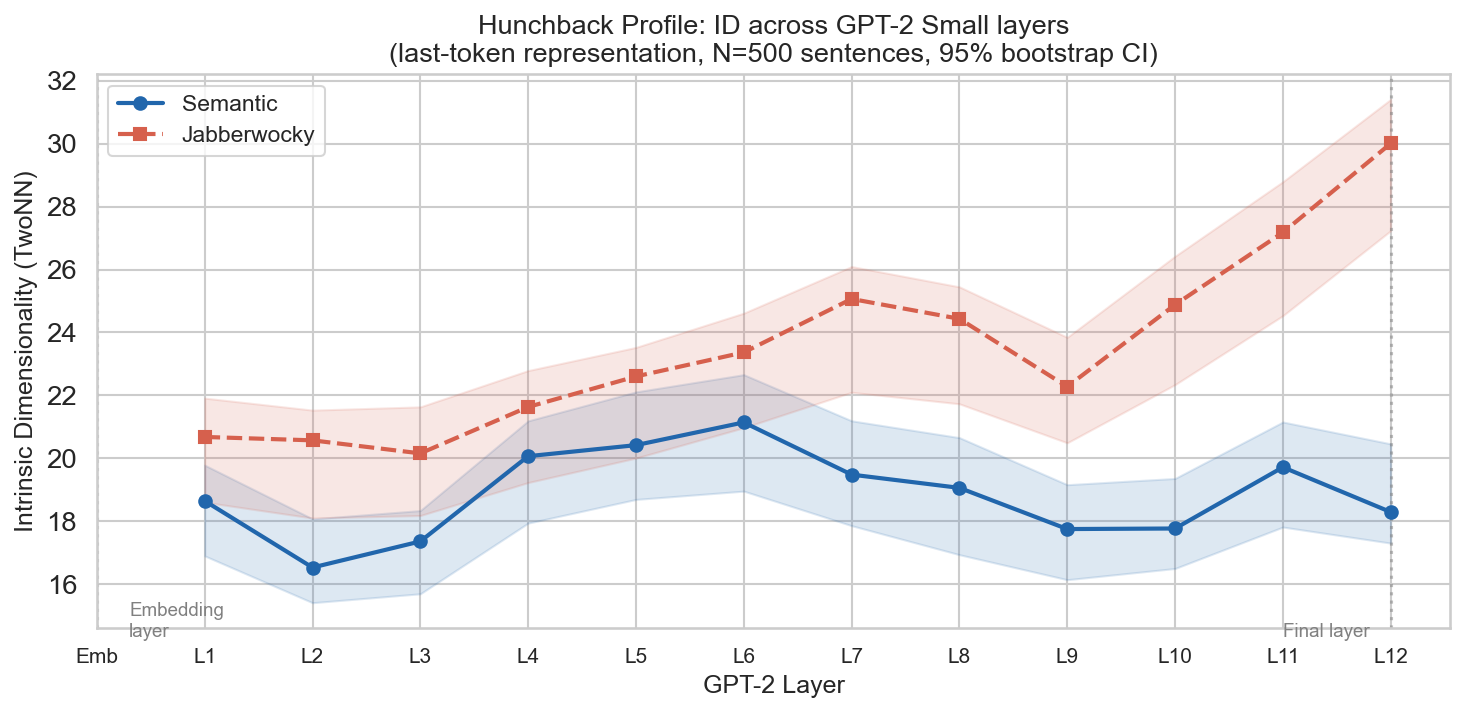
\includegraphics[width=0.85\linewidth]{fig1_hunchback.png}
    \caption{Évolution de la Dimensionnalité Intrinsèque (ID) à travers les couches de GPT-2 Small pour les phrases sémantiques et Jabberwocky (Calcul sur le dernier jeton de la phrase, 1000 itérations de bootstrap sans remise pour l'intervalle de confiance à 95\%).}
    \label{fig:hunchback_results}
\end{figure}

L'analyse de ces profils révèle une divergence spectaculaire entre les deux groupes de stimuli :
\begin{itemize}
    \item \textbf{La condition sémantique (courbe bleue) :} Elle suit fidèlement le profil de « Hunchback » documenté par Ansuini et al. \cite{ansuini2019intrinsic}. L'ID débute à 18.65 à la première couche cachée, augmente jusqu'à atteindre un maximum géométrique à la \textbf{couche 6 (ID = 21.14)} (phase d'expansion où les variables latentes sémantiques sont démêlées), puis décroît de façon monotone jusqu'à **18.29** à la couche de décision finale 12 (phase de compression/abstraction).
    \item \textbf{La condition Jabberwocky (courbe rouge) :} Elle commence à un niveau supérieur (20.68) et, au lieu de décroître après la phase d'expansion, **l'ID continue de croître pour culminer à son maximum à la couche finale 12 (ID = 30.01)**.
\end{itemize}

La différence nette entre les deux conditions ($\Delta\text{ID} = \text{ID}_{\text{semantic}} - \text{ID}_{\text{jabberwocky}}$) est représentée dans la Figure \ref{fig:diff_results}. Elle montre qu'à partir de la couche 7, la représentation du Jabberwocky devient significativement et de plus en plus dispersée par rapport à celle du sémantique.

\begin{figure}[htbp]
    \centering
    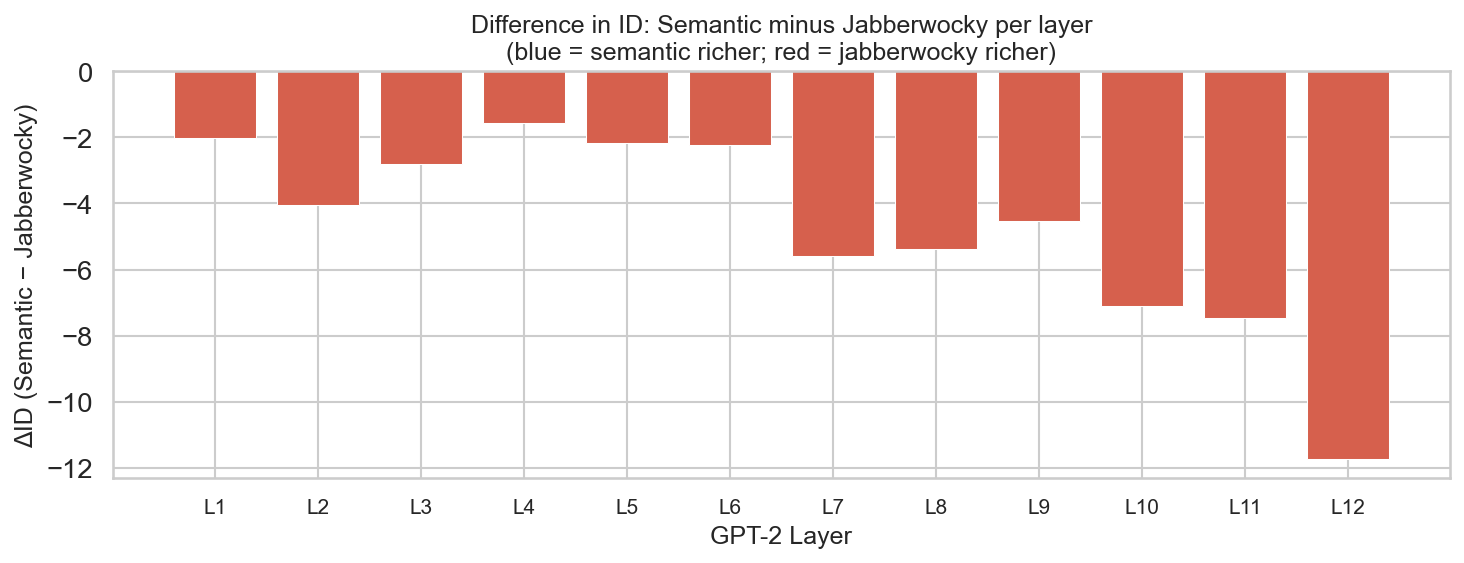
\includegraphics[width=0.8\linewidth]{fig4_id_difference.png}
    \caption{Différence de dimensionnalité intrinsèque ($\Delta\text{ID}$) par couche. Les valeurs négatives indiquent une géométrie plus complexe pour le groupe Jabberwocky.}
    \label{fig:diff_results}
\end{figure}

Ces observations confirment notre **Hypothèse 3** : face à une séquence linguistique qui respecte la syntaxe mais ne porte aucun sens, le modèle ne parvient pas à unifier les concepts dans ses couches supérieures. Faute de pouvoir projeter les données sur une variété sémantique stable et de basse dimension, les représentations finales restent bruitées et dispersées, empêchant la phase de compression géométrique caractéristique des représentations cohérentes.

\section{Dynamique Temporelle au cours de la Phrase : Ramping}
Le deuxième axe d'analyse porte sur l'intégration incrémentale de l'information au cours de la lecture. Nous avons calculé l'ID locale pour chacun des 10 déciles de position des phrases en extrayant un token représentatif unique par décile afin de préserver l'indépendance statistique des points.

Les profils de ramping pour des couches clés (les couches 3, 6, 9 et la couche finale 12) sont illustrés par la Figure \ref{fig:ramping_results}.

\begin{figure}[htbp]
    \centering
    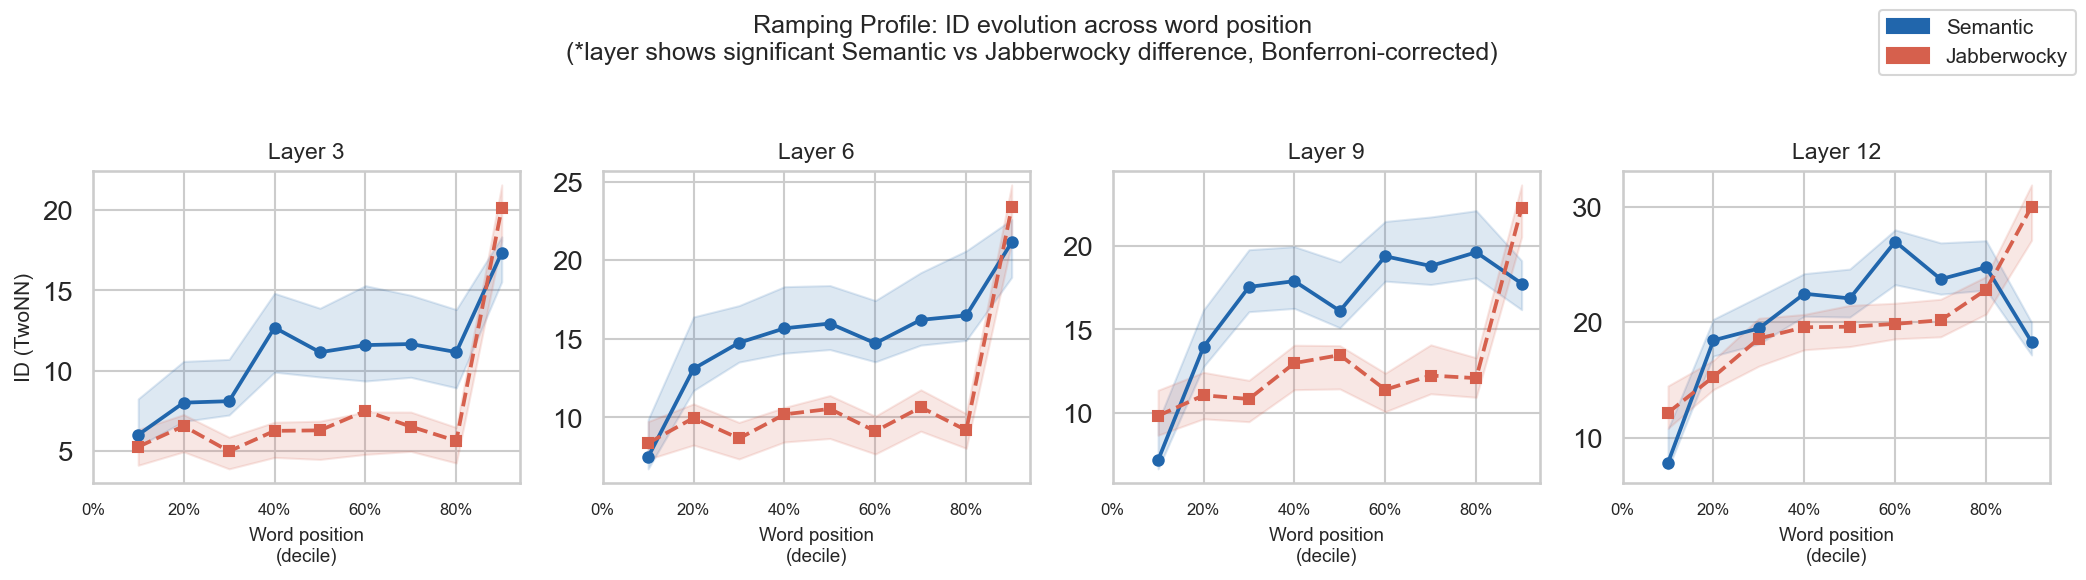
\includegraphics[width=0.95\linewidth]{fig2_ramping.png}
    \caption{Évolution temporelle de la dimensionnalité intrinsèque (ramping par décile de position des mots) pour différentes couches. L'étoile (*) signale une différence significative entre sémantique et Jabberwocky ($p < 0.05$ après correction de Bonferroni).}
    \label{fig:ramping_results}
\end{figure}

Les analyses de régression de la pente de ramping révèlent des caractéristiques temporelles distinctives :
\begin{itemize}
    \item \textbf{Dans le groupe sémantique : } Des pentes positives et statistiquement significatives ($p < 0.05$) sont détectées dès la **couche 3** ($\text{pente} = 1.02, R^2 = 0.72$) et se maintiennent de manière robuste jusqu'à la couche 11. Cette augmentation lente et continue de la dimensionnalité géométrique confirme l'existence d'un processus incrémental d'intégration contextuelle.
    \item \textbf{Dans le groupe Jabberwocky : } Aucune pente significative n'est mesurée dans les couches basses ou intermédiaires (couches 3 à 8). En revanche, un ramping tardif et brutal est mesuré aux couches de sortie, culminant à la **couche 12** ($\text{pente} = 1.62, R^2 = 0.82, p < 0.001$).
\end{itemize}

Ce résultat valide nos \textbf{Hypothèses 1 et 2}. 

De plus, l'observation fine de la trajectoire du Jabberwocky (par exemple à la couche 9, voir Figure \ref{fig:ramping_results}) montre que l'ID reste particulièrement basse et stable du décile 10\% au décile 80\% (aux alentours de 11--13) avant de subir une hausse spectaculaire et soudaine au décile 90\% (atteignant 22.28). Ce comportement traduit deux phases cognitives distinctes chez le modèle :
\begin{itemize}
    \item \textbf{Le «~holding pattern~» syntaxique (déciles 10\% à 80\%) :} Ne pouvant pas unifier de concepts sémantiques puisque les mots sont dénués de sens, le modèle se contente de maintenir en mémoire de travail les relations purement syntaxiques et grammaticales locales. Ce stockage structurel est peu coûteux en paramètres et conserve les représentations sur une sous-variété de basse dimensionnalité stable.
    \item \textbf{Le goulot d'intégration de fin de phrase (décile 90\%) :} Au niveau du dernier mot et de la ponctuation finale, le modèle causal est contraint de fermer la proposition syntaxique et d'intégrer l'ensemble de la séquence afin de prédire la suite. Ce traitement fait écho au phénomène de \textit{clause wrap-up} documenté en psycholinguistique par Just et Carpenter \cite{just1980theory}, qui met en évidence un surcoût cognitif d'intégration à la frontière des phrases. Chez le modèle de langage, ce goulot d'unification se concentre géométriquement sur le point final, qui agit comme un puits d'attention (\textit{attention sink}) compilant la représentation globale de la séquence \cite{clark2019what}. Face à l'impossibilité d'associer ces pseudo-mots dans un concept sémantique unifié pré-existant, cette intégration finale échoue à compresser l'information et provoque une dispersion géométrique immédiate des vecteurs, d'où le bond soudain de la dimensionnalité.
\end{itemize}

Le ramping de l'ID, signature géométrique de l'unification sémantique, est donc précoce et progressif pour les phrases cohérentes. Pour le Jabberwocky, il est remplacé par une stabilité syntaxique transitoire suivie d'une rupture dimensionnelle brutale à la frontière de la phrase.

\section{Impact Technique de la Tokenisation (BPE)}
Avant d'entamer la discussion de ces résultats, il est essentiel d'examiner le rôle joué par l'algorithme de tokenisation Byte Pair Encoding (BPE). Les pseudo-mots n'appartenant pas au vocabulaire d'apprentissage de GPT-2 Small, ils subissent une fragmentation en sous-tokens. La Figure \ref{fig:bpe_results} représente la distribution du ratio de longueur de tokenisation entre nos paires de stimuli.

\begin{figure}[htbp]
    \centering
    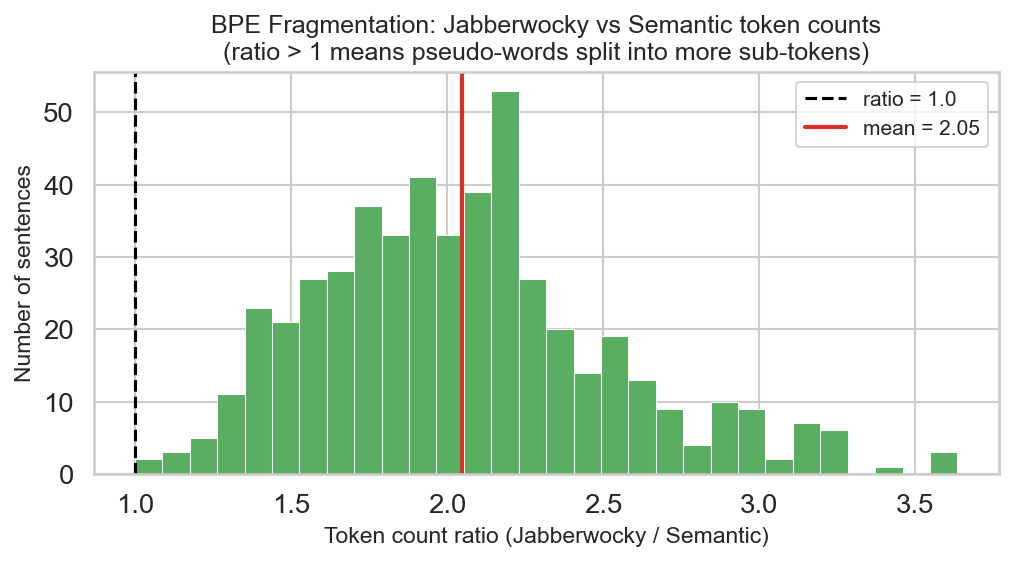
\includegraphics[width=0.75\linewidth]{fig3_bpe_fragmentation.png}
    \caption{Distribution du ratio de fragmentation BPE (Jabberwocky / Sémantique).}
    \label{fig:bpe_results}
\end{figure}

Le Jabberwocky comporte en moyenne **2.05 fois plus de tokens** que les phrases naturelles équivalentes. Cette fragmentation accrue signifie que le modèle de langage causal effectue plus d'étapes d'auto-attention pour le Jabberwocky. Notre choix d'extraire exactement un mot-frontière par décile de progression s'avère donc crucial : il a permis de normaliser le pas de temps expérimental et de garantir que la différence de ramping sémantique/Jabberwocky observée ne soit pas un simple artefact du nombre de tokens traités par le modèle.

\section{Discussion et Parallèles Neurolinguistiques}
La confrontation de nos résultats théoriques et empiriques avec le modèle neurolinguistique MUC (Memory, Unification, Control) permet d'établir plusieurs parallèles constructifs :

\subsection{L'Unification comme accumulation dimensionnelle}
Dans le cerveau humain, le processus d'unification (localisé dans le gyrus frontal inférieur gauche, ou aire de Broca) assemble dynamiquement les informations lexicales récupérées de la mémoire (cortex temporal) pour construire le sens global de la phrase. Fedorenko et al. \cite{fedorenko2016broad} ont montré que l'activité électrique de cette région augmente continuellement au cours de la lecture d'une phrase porteuse de sens, reflétant une charge de traitement croissante, un signal absent pour le Jabberwocky.

Nos résultats indiquent une dynamique similaire au sein de GPT-2 Small. Le ramping progressif de la dimensionnalité intrinsèque dans les couches intermédiaires (couches 3 à 8) s'apparente à cette charge computationnelle d'unification. L'espace géométrique des embeddings de GPT-2 s'élargit temporairement pour structurer et unifier les variables linguistiques sémantiques au fur et à mesure que le contexte se densifie.

\subsection{Absence de Contrôle et explosion de dimension}
Une différence critique demeure toutefois entre le cerveau humain et le réseau neuronal artificiel. Face à du Jabberwocky, les humains désengagent rapidement leur attention sémantique après avoir constaté l'incohérence, limitant la charge d'unification (d'où l'absence de ramping dans les observations de Fedorenko et al.). Ce rôle de régulation attentionnelle est attribué à la composante de **Contrôle** du modèle MUC, localisée dans le cortex préfrontal dorsolatéral.

À l'inverse, GPT-2 Small est dépourvu de mécanisme de contrôle cognitif. En tant que modèle statistique autoregressif, il est contraint d'appliquer le même traitement causal uniforme à toute entrée. Face à des phrases Jabberwocky, le modèle ne peut "abandonner" la recherche de sens. Il tente d'associer des variables sémantiques incompatibles sur des pseudo-mots fragmentés, ce qui conduit à cette explosion de l'ID dans les dernières couches cachées (ID = 30.01 à la couche 12). Cette absence de contrôle explique pourquoi le profil Hunchback s'effondre en fin de réseau pour le Jabberwocky, le modèle restant piégé dans un espace de représentation de haute complexité faute de pouvoir converger vers un concept abstrait.
